\chapter{VLANs: Part 2}\label{vlans-part-2}

Basic VLAN topology from PART 1

\begin{figure}
\centering
\pandocbounded{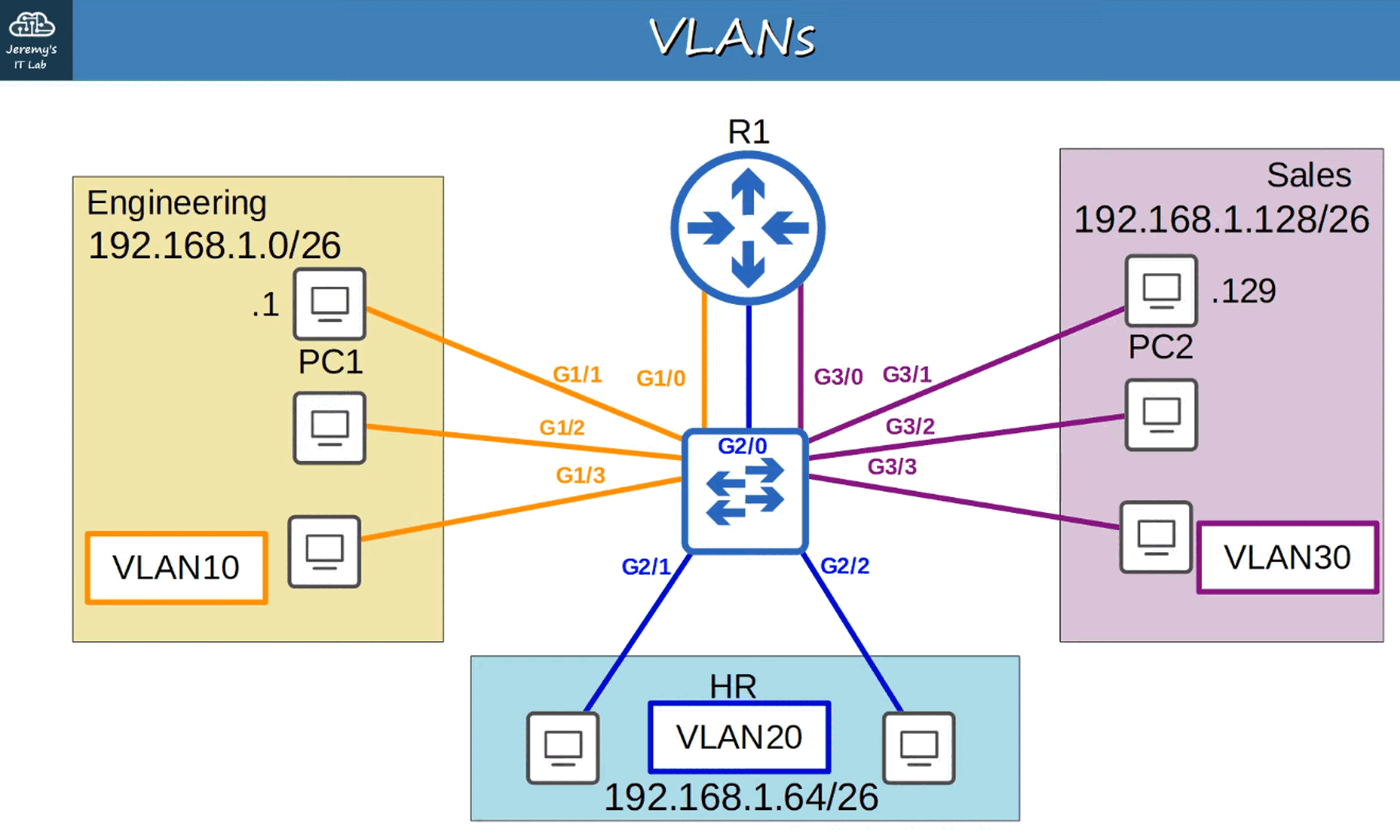
\includegraphics[keepaspectratio,alt={image}]{images/18-vlan-part2/img-001.png}}
\end{figure}

What about THIS Network Topology ?

\begin{figure}
\centering
\pandocbounded{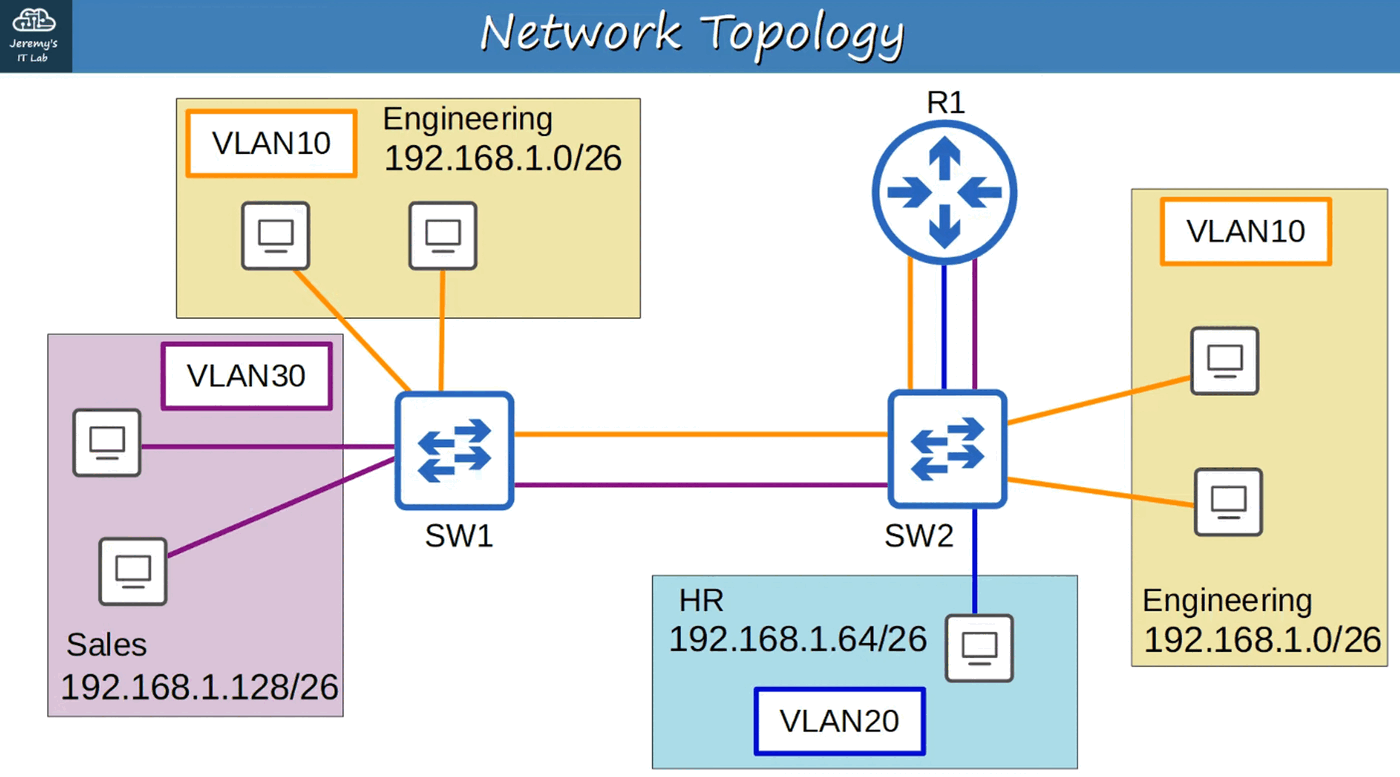
\includegraphics[keepaspectratio,alt={image}]{images/18-vlan-part2/img-002.png}}
\end{figure}

Notice this one has TWO Switches (SW1 and SW2) and ENGINEERING (VLAN 10)
has two separate locations on the network.

\section{Trunk Ports}\label{trunk-ports}

\begin{itemize}
\item
  In a small network with few VLANS, it's possible to use a separate
  interface for EACH VLAN when connecting SWITCHES to SWITCHES, and
  SWITCHES to ROUTERS
\item
  HOWEVER, when the number of VLANS increases, this is not viable. It
  will result in wasted interfaces, and often ROUTERS won't have enough
  INTERFACES for each VLAN
\item
  You can use TRUNK PORTS to carry traffic from multiple VLANS over a
  single interface
\end{itemize}

A TRUNK PORT carrying multiple VLAN connections over single interface

\begin{figure}
\centering
\pandocbounded{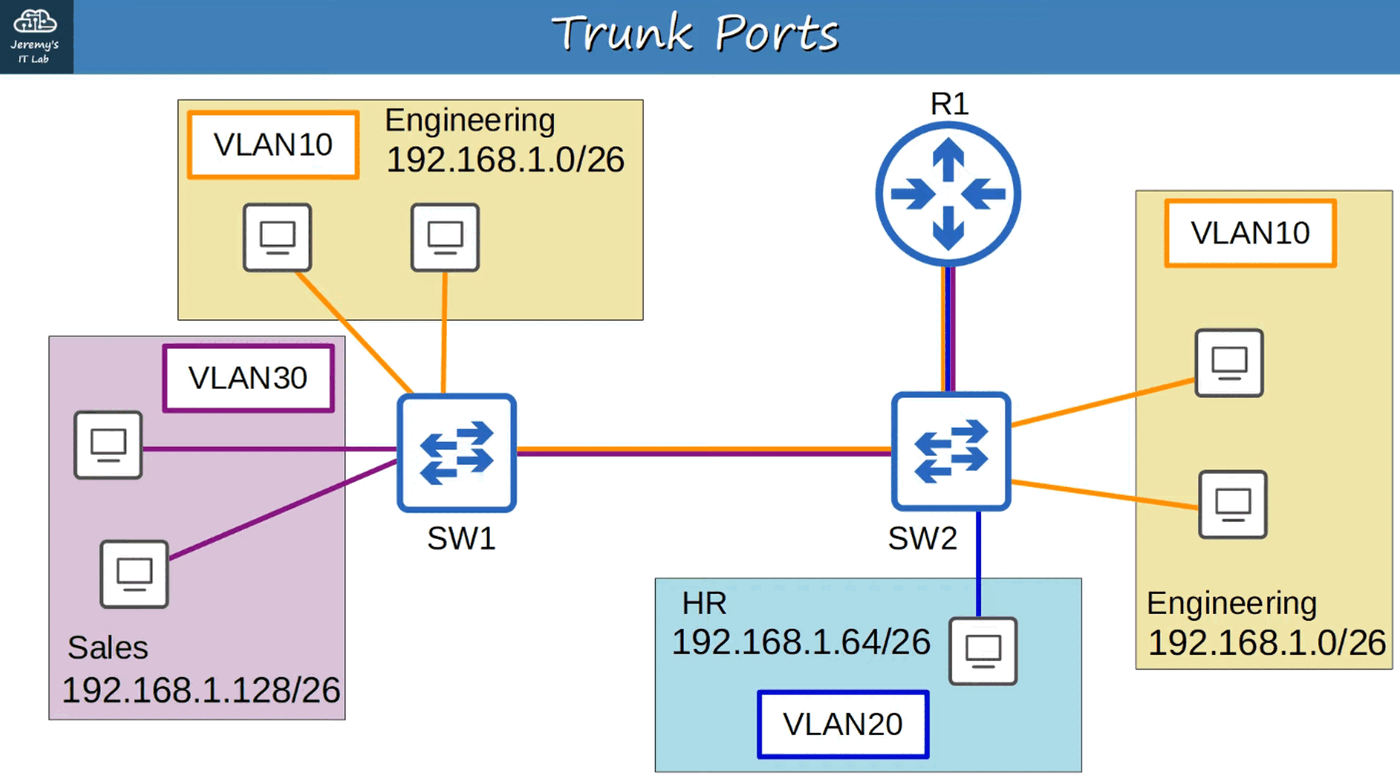
\includegraphics[keepaspectratio,alt={image}]{images/18-vlan-part2/img-003.png}}
\end{figure}

\begin{figure}
\centering
\pandocbounded{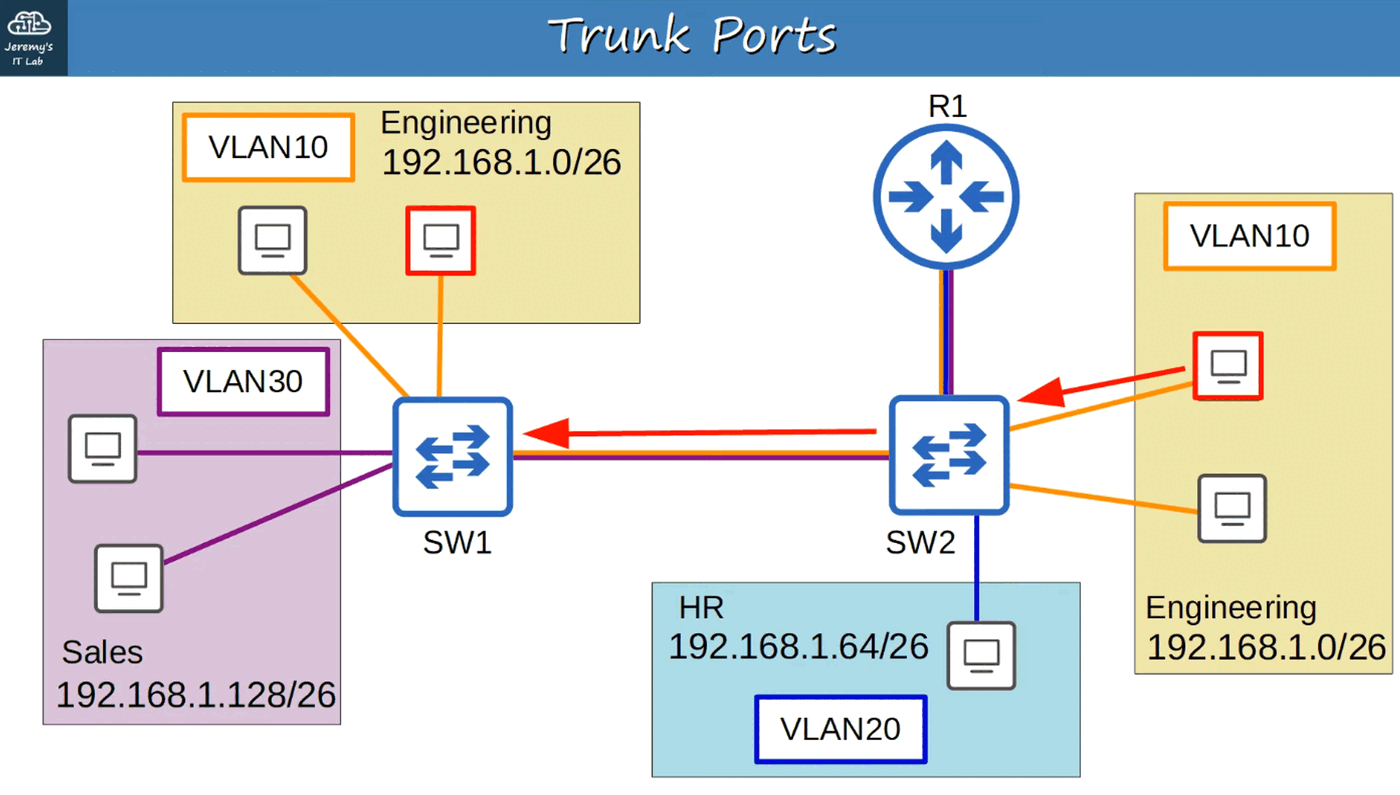
\includegraphics[keepaspectratio,alt={image}]{images/18-vlan-part2/img-004.png}}
\end{figure}

How does a packet know WHICH VLAN to send traffic to over the TRUNK PORT
?

VLAN TAGS !

SWITCHES will ``tag'' all frames that they send over a TRUNK LINK. This
allows the receiving SWITCH to know which VLAN the frame belongs to.

TRUNK PORT = ``Tagged'' ports

ACCESS PORT = ``Untagged'' ports

\section{VLAN Tagging}\label{vlan-tagging}

\begin{itemize}
\tightlist
\item
  There are TWO main TRUNK protocols:

  \begin{itemize}
  \tightlist
  \item
    ISL (Inter-Switch Link)
  \item
    IEEE 802.1Q (also known as ``dot1q'')
  \end{itemize}
\end{itemize}

ISL is an old Cisco proprietary protocol created before industry
standard IEEE 802.1Q

IEEE 802.1Q is an industry standard protocol created by the IEEE
(Institute of Electrical and Electronics Engineers)

You will probably NEVER use ISL in the real world; even modern Cisco
equipment doesn't use it.

For the CCNA, you will only need to learn 802.1Q

ETHERNET HEADER with 802.1Q

\begin{figure}
\centering
\pandocbounded{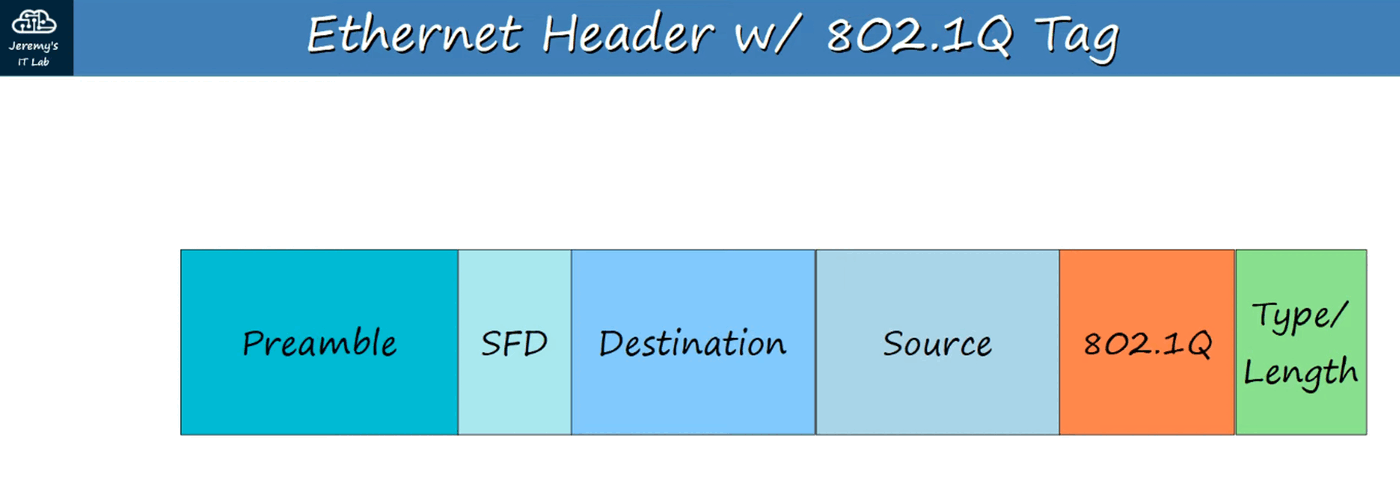
\includegraphics[keepaspectratio,alt={image}]{images/18-vlan-part2/img-005.png}}
\end{figure}

\begin{itemize}
\tightlist
\item
  The 802.1Q TAG Is inserted between the SOURCE and TYPE/LENGTH fields
  in the ETHERNET FRAME
\item
  The TAG is 4 bytes (32 bits) in length
\item
  The TAG consists of TWO main fields:

  \begin{itemize}
  \tightlist
  \item
    Tag Protocol Identifier (TPID)
  \item
    Tag Control Information (TCI)

    \begin{itemize}
    \tightlist
    \item
      TCI consists of THREE sub-fields:
    \end{itemize}
  \end{itemize}
\end{itemize}

\begin{figure}
\centering
\pandocbounded{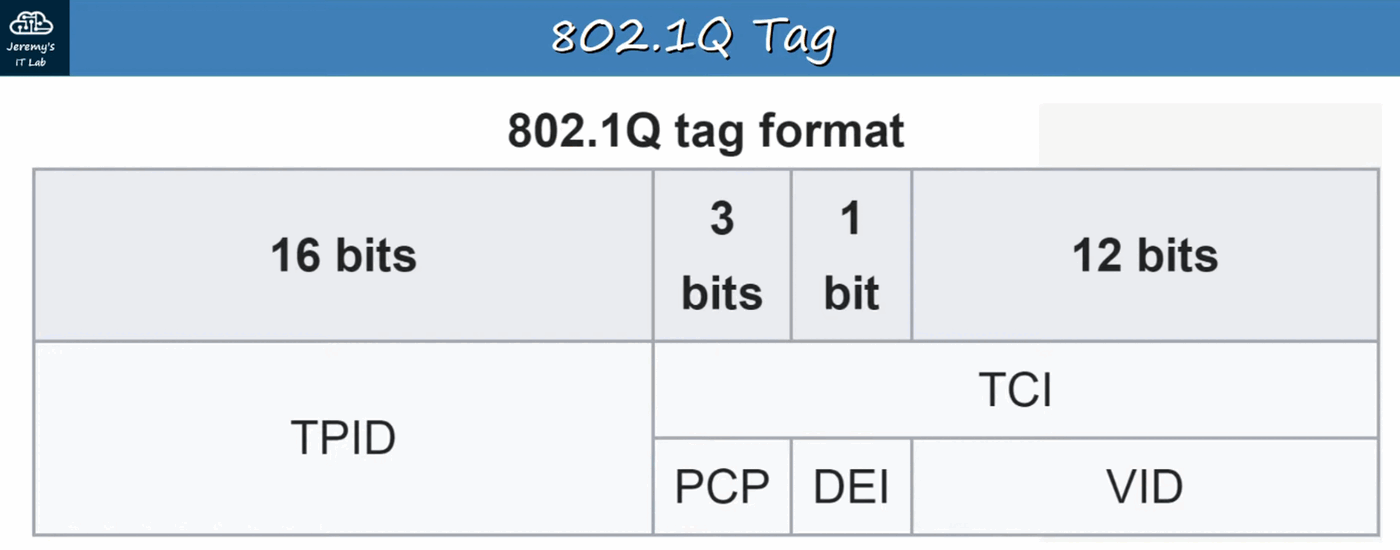
\includegraphics[keepaspectratio,alt={image}]{images/18-vlan-part2/img-006.png}}
\end{figure}

TPID (TAG Protocol Identifier) :

\begin{itemize}
\tightlist
\item
  16 bits (2 bytes) in length
\item
  Always set to a value of 0x8100. This indicates that the frame is
  802.1Q TAG
\end{itemize}

TCI / PCP (Priority Code Point) :

\begin{itemize}
\tightlist
\item
  3 bits in length
\item
  Used for Class of Service (CoS), which prioritizes important traffic
  in congested networks
\end{itemize}

TCI / DEI (Drop Eligible Indicator) :

\begin{itemize}
\tightlist
\item
  1 bit in length
\item
  Used to indicated frames that can be dropped if the network is
  congested
\end{itemize}

\section{TCI / VID (VLAN ID)}\label{tci-vid-vlan-id}

\begin{itemize}
\tightlist
\item
  12 bits in length
\item
  Identifies the VLAN the frame belongs to
\item
  12 bits in length = 4096 total VLANS (2\^{}12), range of 0 - 4095
\item
  VLANs 0 and 4095 are reserved and can't be used
\item
  Therefore, the actual range of VLANs is 1 - 4094
\end{itemize}

NOTE : Cisco's ISL also had a VLAN range of 1 - 4094

\section{VLAN Ranges}\label{vlan-ranges}

\begin{figure}
\centering
\pandocbounded{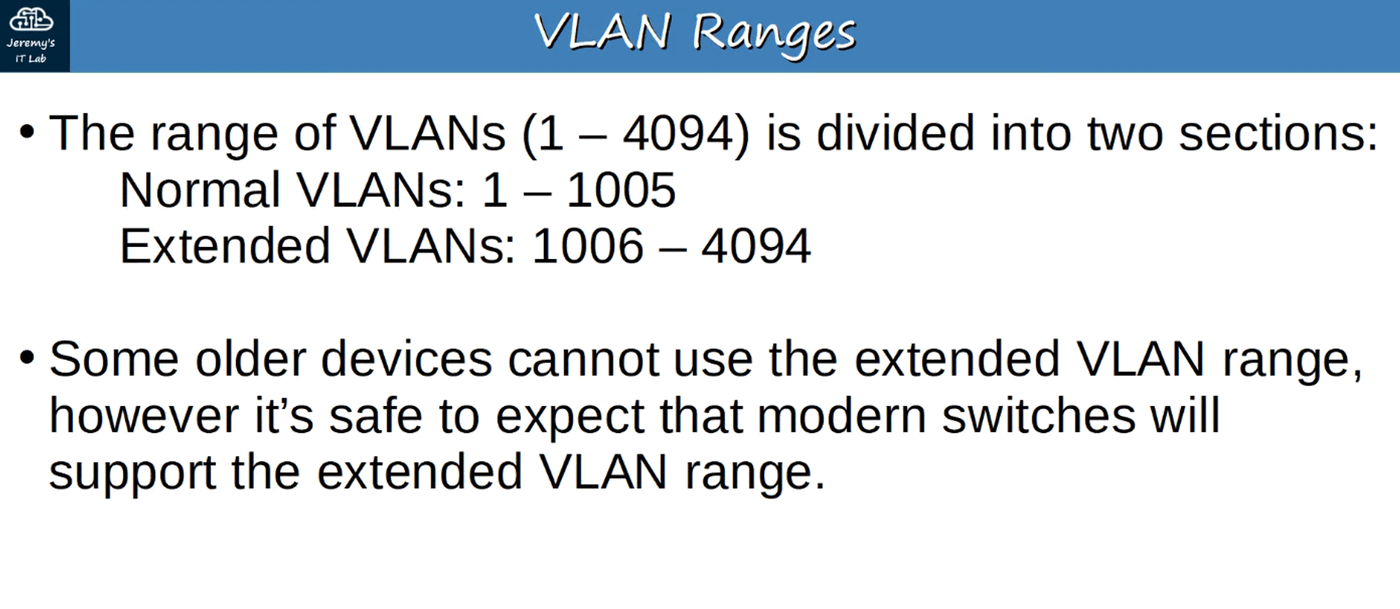
\includegraphics[keepaspectratio,alt={image}]{images/18-vlan-part2/img-007.png}}
\end{figure}

\section{Native VLAN}\label{native-vlan}

\begin{figure}
\centering
\pandocbounded{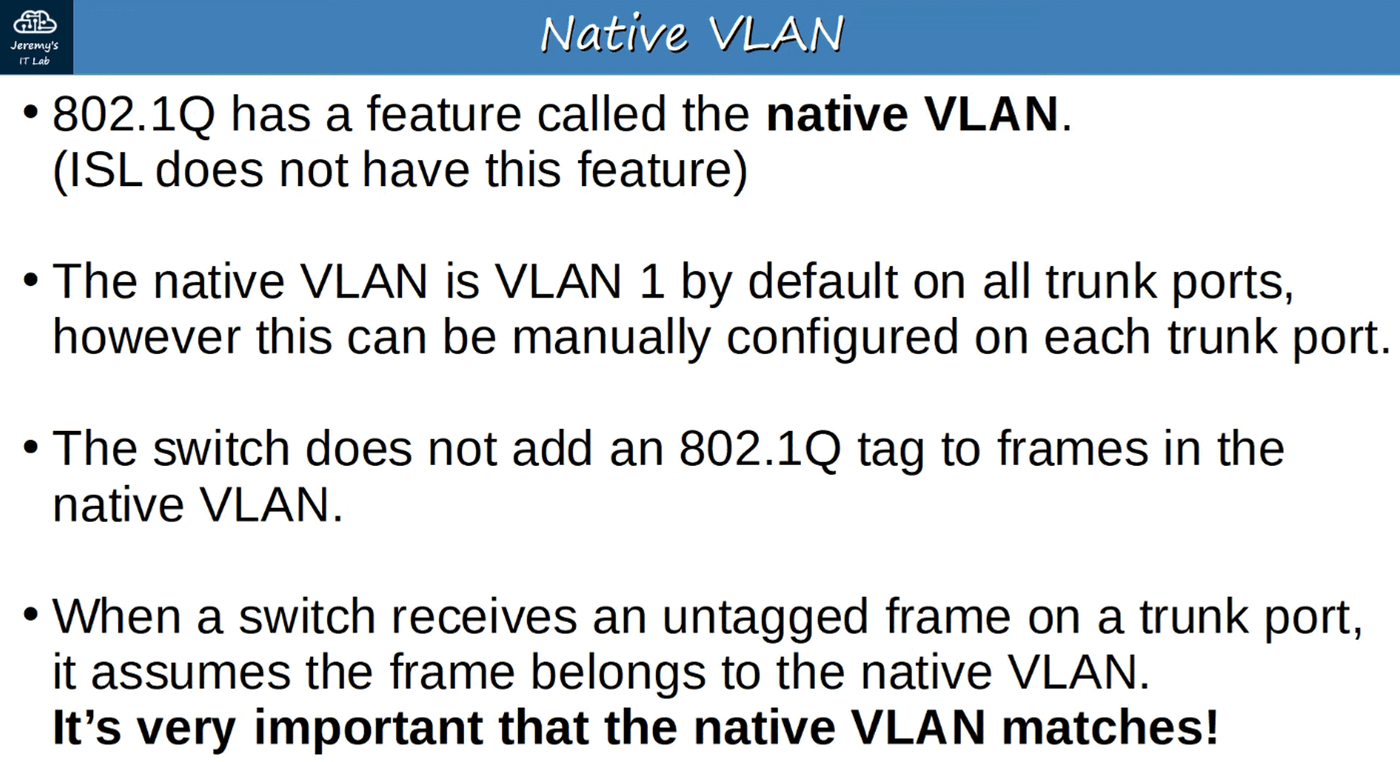
\includegraphics[keepaspectratio,alt={image}]{images/18-vlan-part2/img-008.png}}
\end{figure}

\begin{figure}
\centering
\pandocbounded{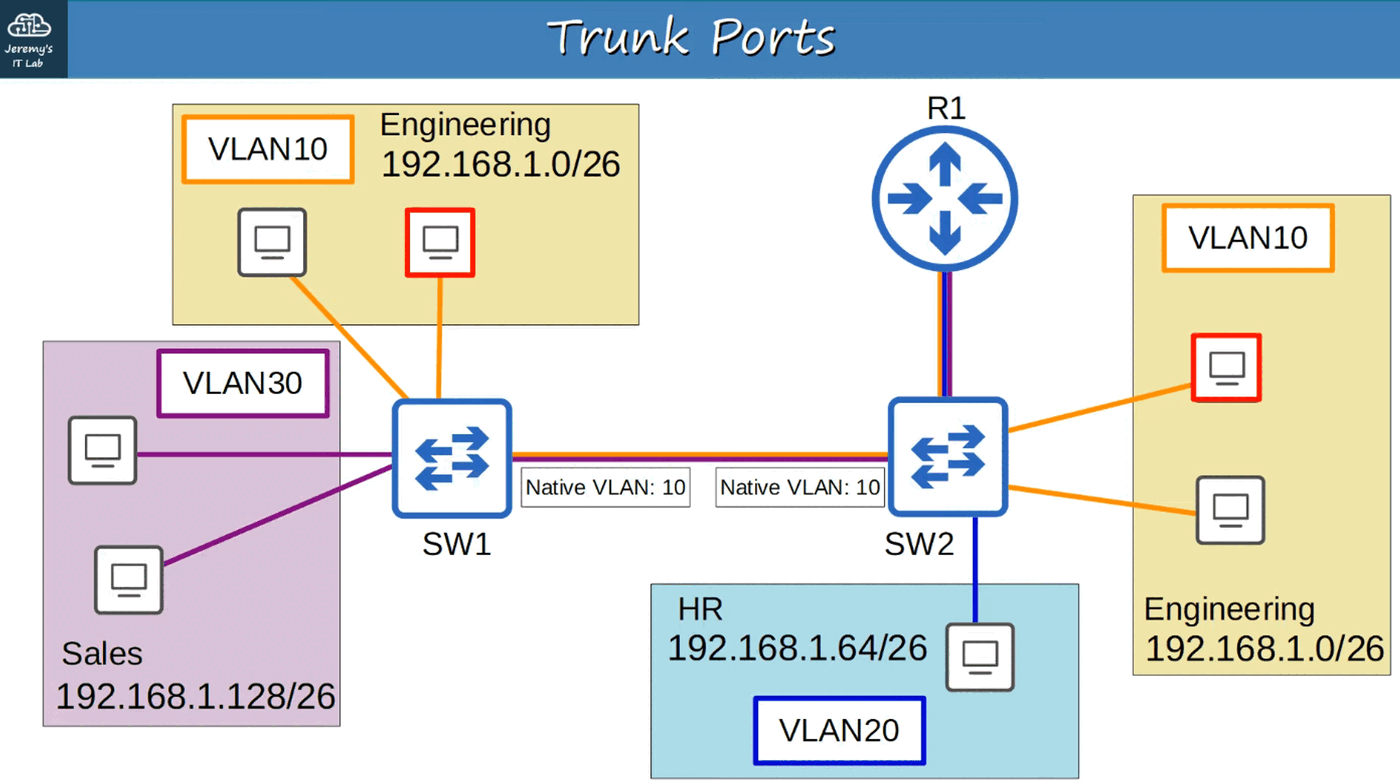
\includegraphics[keepaspectratio,alt={image}]{images/18-vlan-part2/img-009.png}}
\end{figure}

\begin{figure}
\centering
\pandocbounded{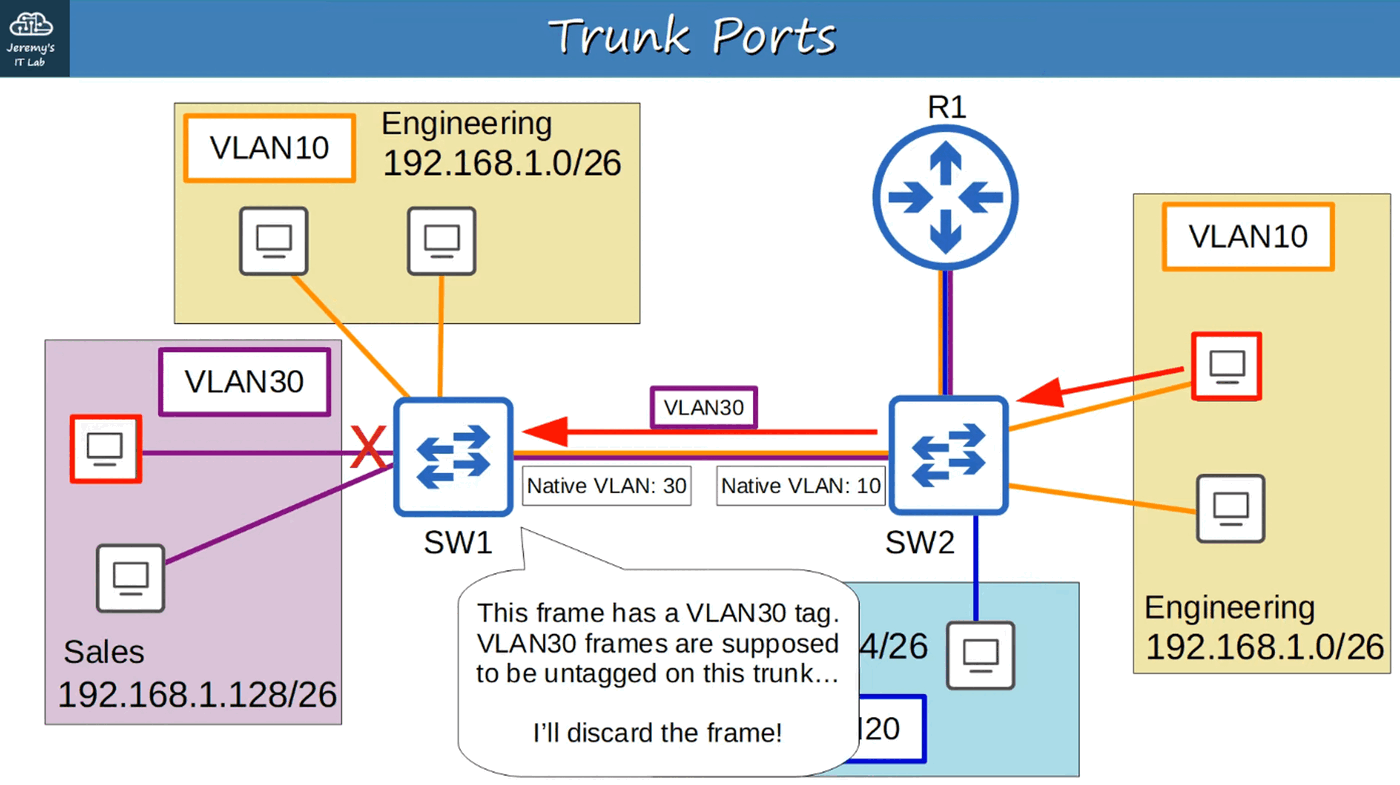
\includegraphics[keepaspectratio,alt={image}]{images/18-vlan-part2/img-010.png}}
\end{figure}

\section{Trunk Configuration}\label{trunk-configuration}

\begin{figure}
\centering
\pandocbounded{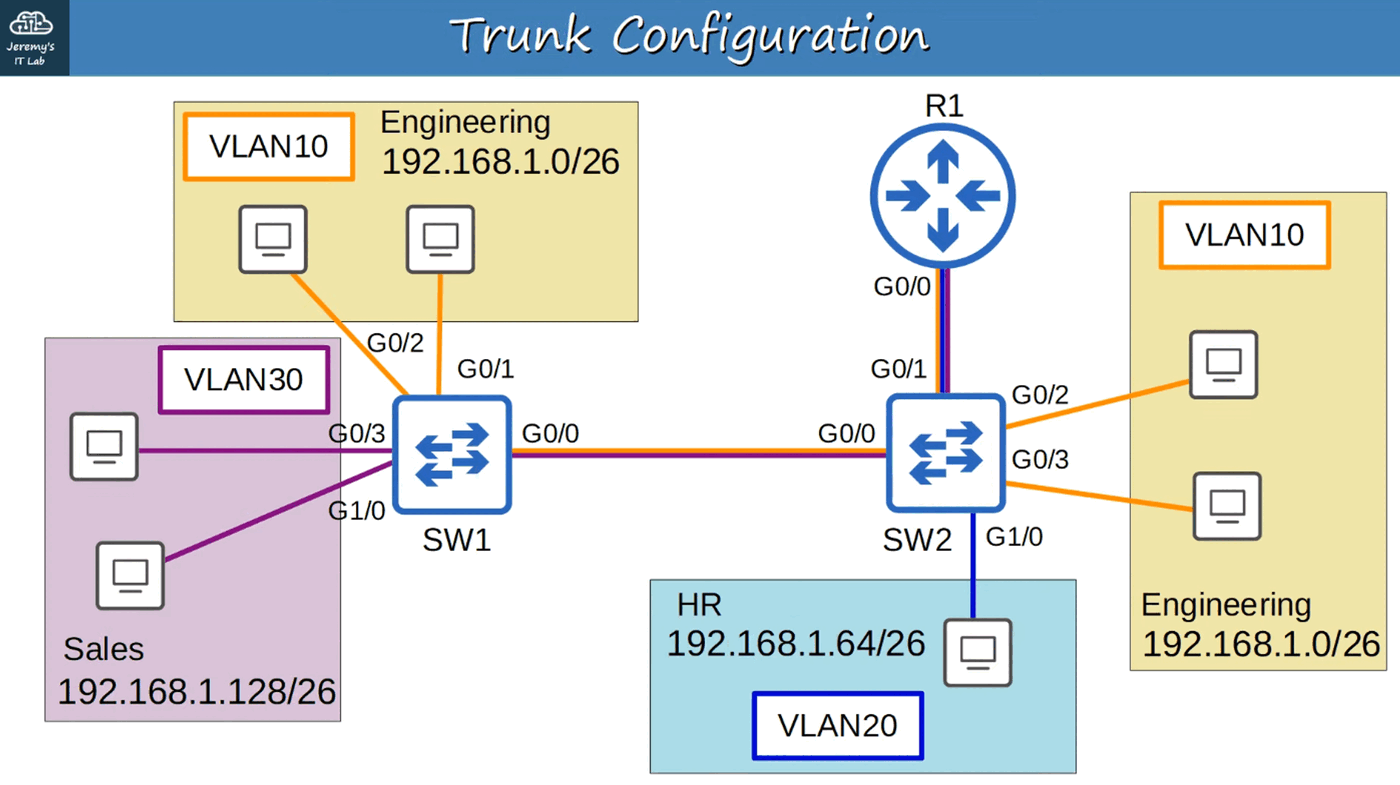
\includegraphics[keepaspectratio,alt={image}]{images/18-vlan-part2/img-011.png}}
\end{figure}

\begin{figure}
\centering
\pandocbounded{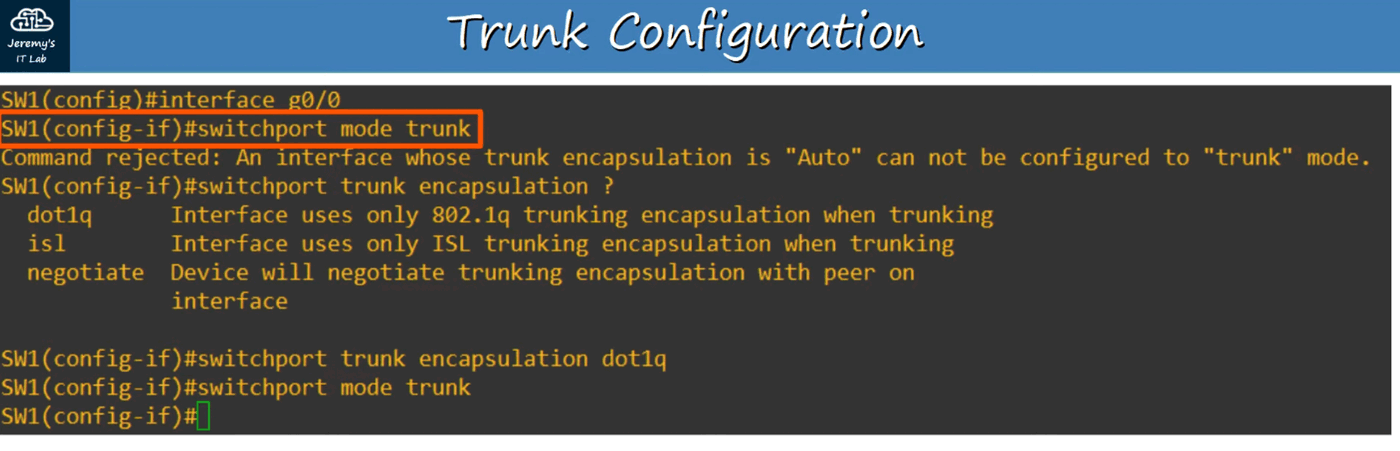
\includegraphics[keepaspectratio,alt={image}]{images/18-vlan-part2/img-012.png}}
\end{figure}

Many modern switches do not support Cisco's ISL at all. They only
support 802.1Q (dot1q)

However, SWITCHES that do support both (like the one I am using in this
example) have a TRUNK encapsulation of ``AUTO'' by default

To MANUALLY configure the INTERFACE as a TRUNK PORT, you must first set
the encapsulation to ``802.1Q'' or ``ISL''. On SWITCHES that only
support 802.1Q, this is not necessary

After you set the encapsulation type, you can then configure the
interface as a TRUNK

\begin{enumerate}
\def\labelenumi{\arabic{enumi})}
\item
  Select the interface to configure
\item
  Use ``\#switchport trunk encapsulation dot1q'' to set the
  encapsulation mode to 802.1Q
\item
  Use ``\#switchport mode trunk'' to manually configure the interface to
  TRUNK
\end{enumerate}

\begin{figure}
\centering
\pandocbounded{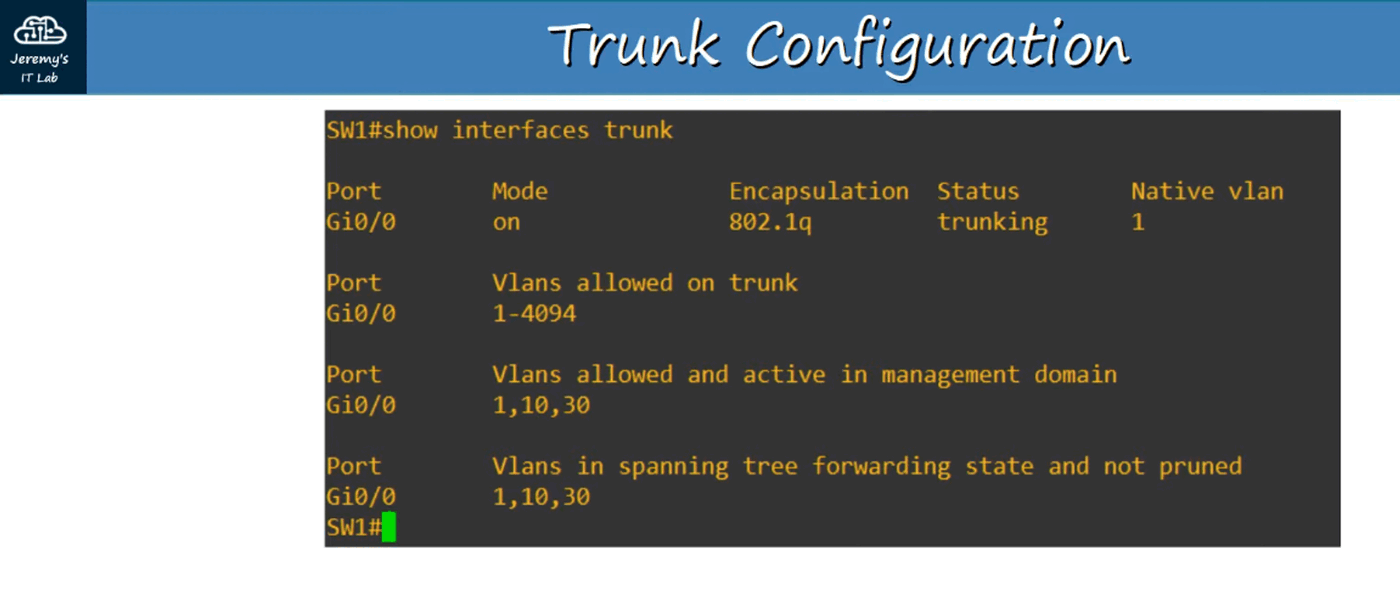
\includegraphics[keepaspectratio,alt={image}]{images/18-vlan-part2/img-013.png}}
\end{figure}

Use the ``\#show interfaces trunk'' command to confirm INTERFACES on
TRUNK

\begin{figure}
\centering
\pandocbounded{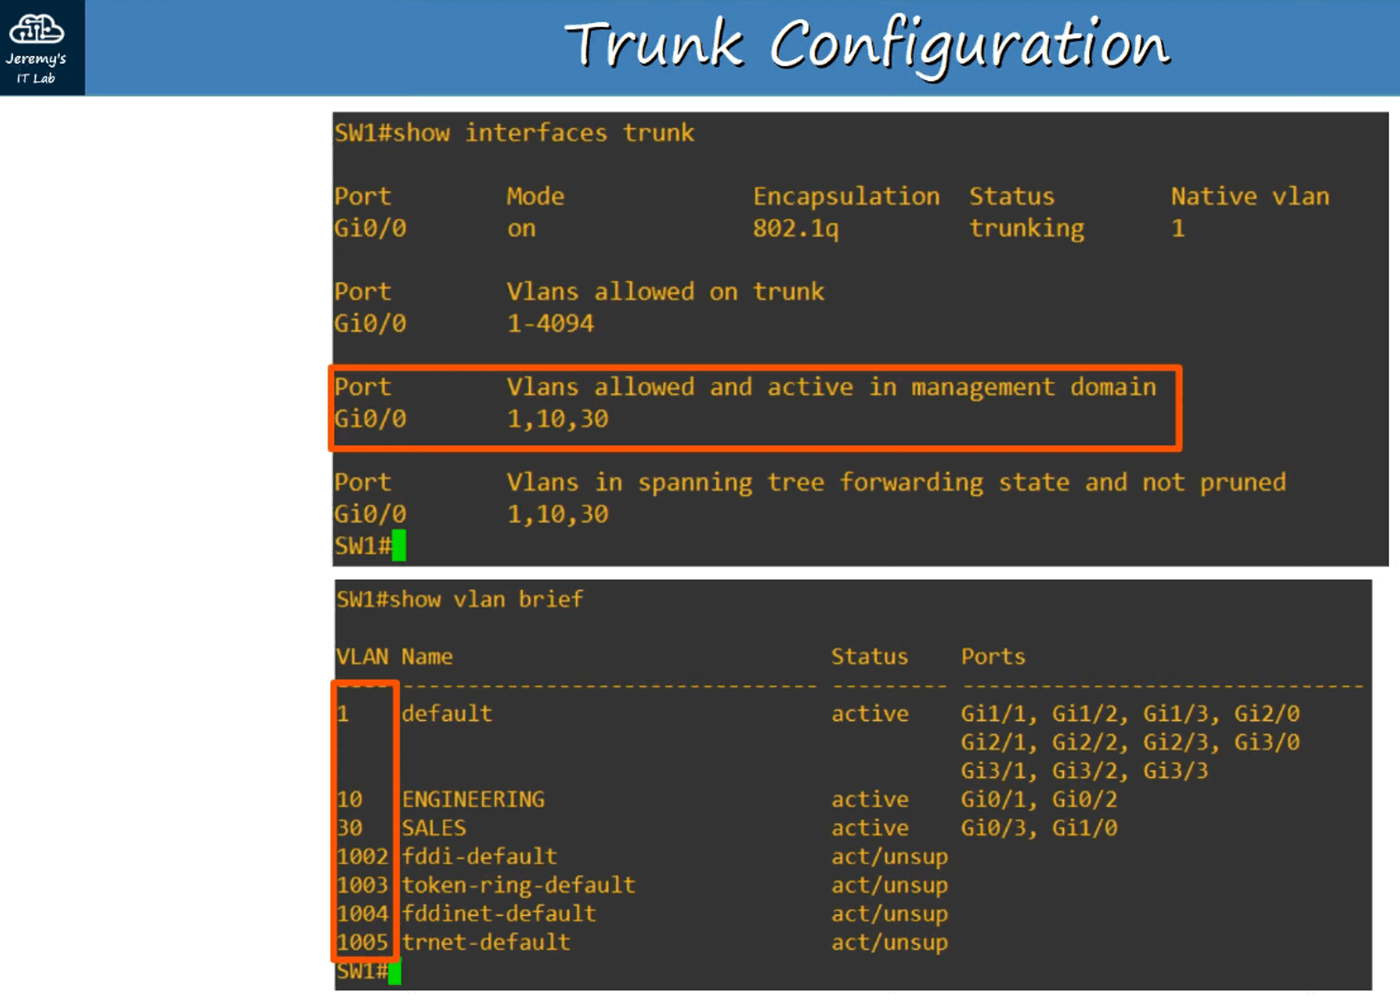
\includegraphics[keepaspectratio,alt={image}]{images/18-vlan-part2/img-014.png}}
\end{figure}

Commands to allow a VLAN on a given TRUNK

\begin{figure}
\centering
\pandocbounded{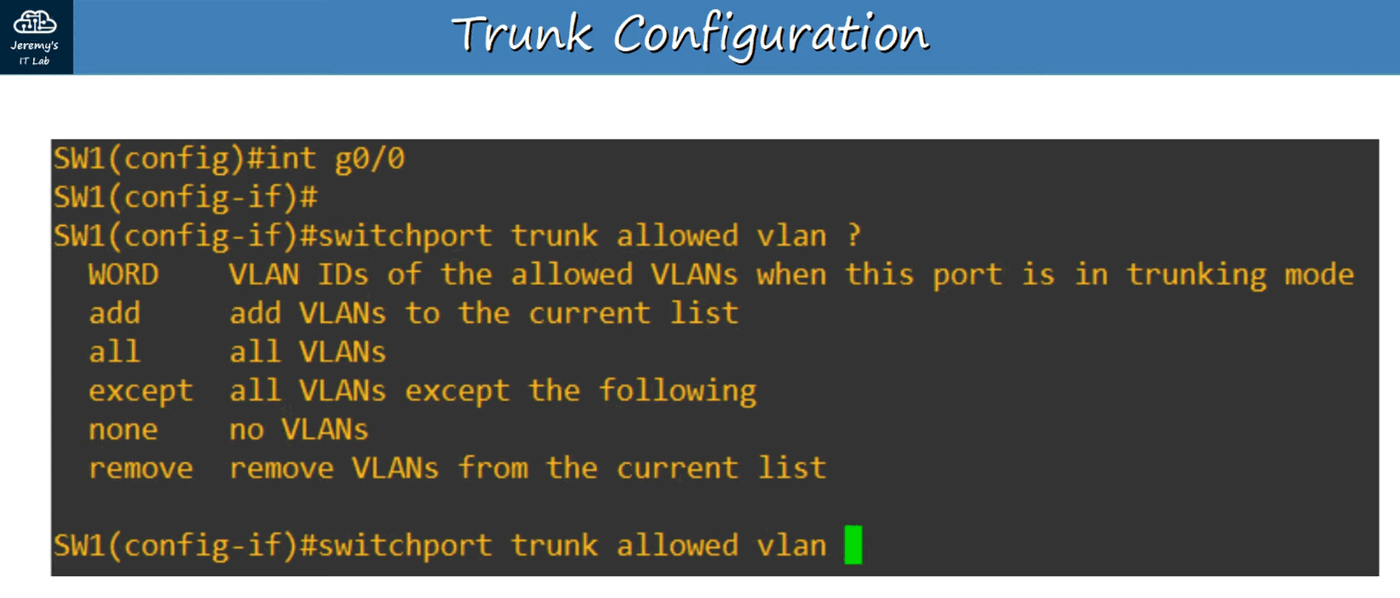
\includegraphics[keepaspectratio,alt={image}]{images/18-vlan-part2/img-015.png}}
\end{figure}

\begin{figure}
\centering
\pandocbounded{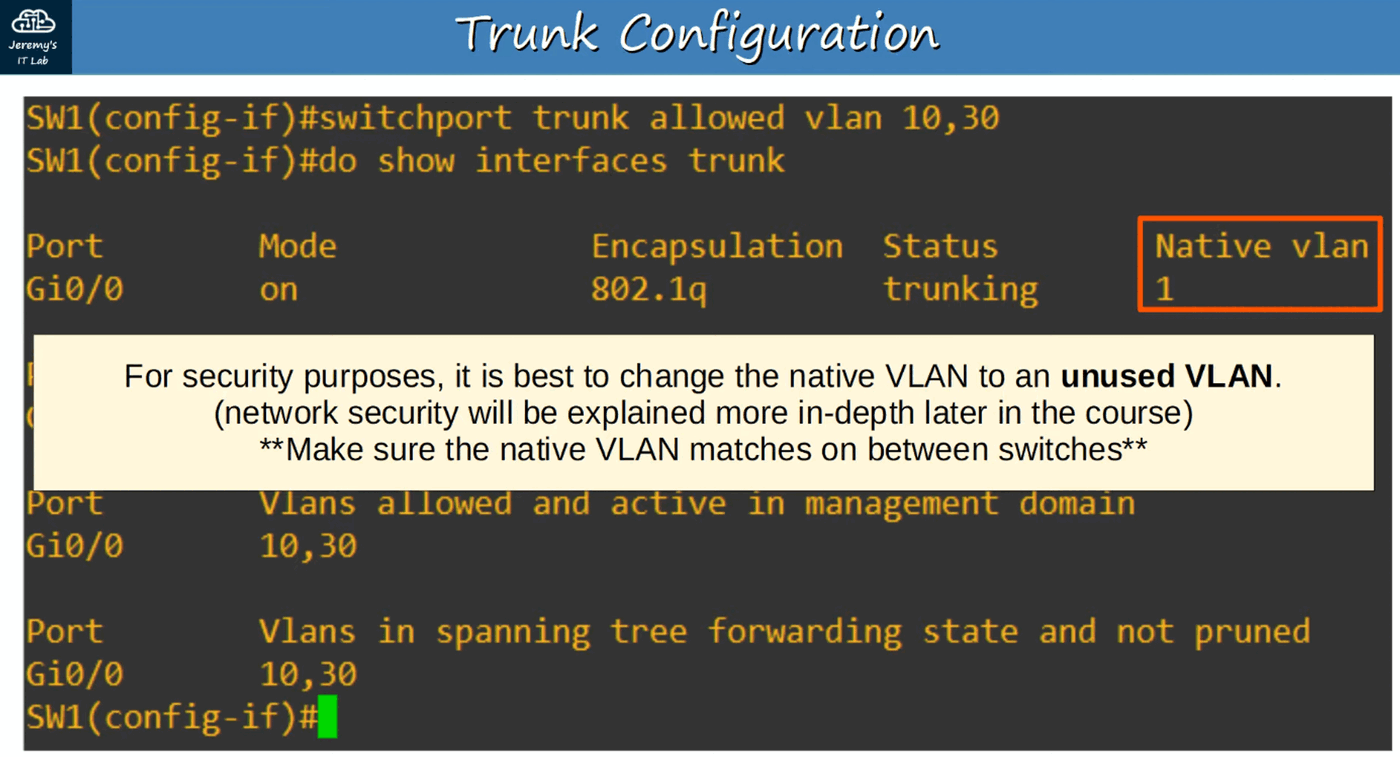
\includegraphics[keepaspectratio,alt={image}]{images/18-vlan-part2/img-016.png}}
\end{figure}

Command to change the NATIVE VLAN

\begin{figure}
\centering
\pandocbounded{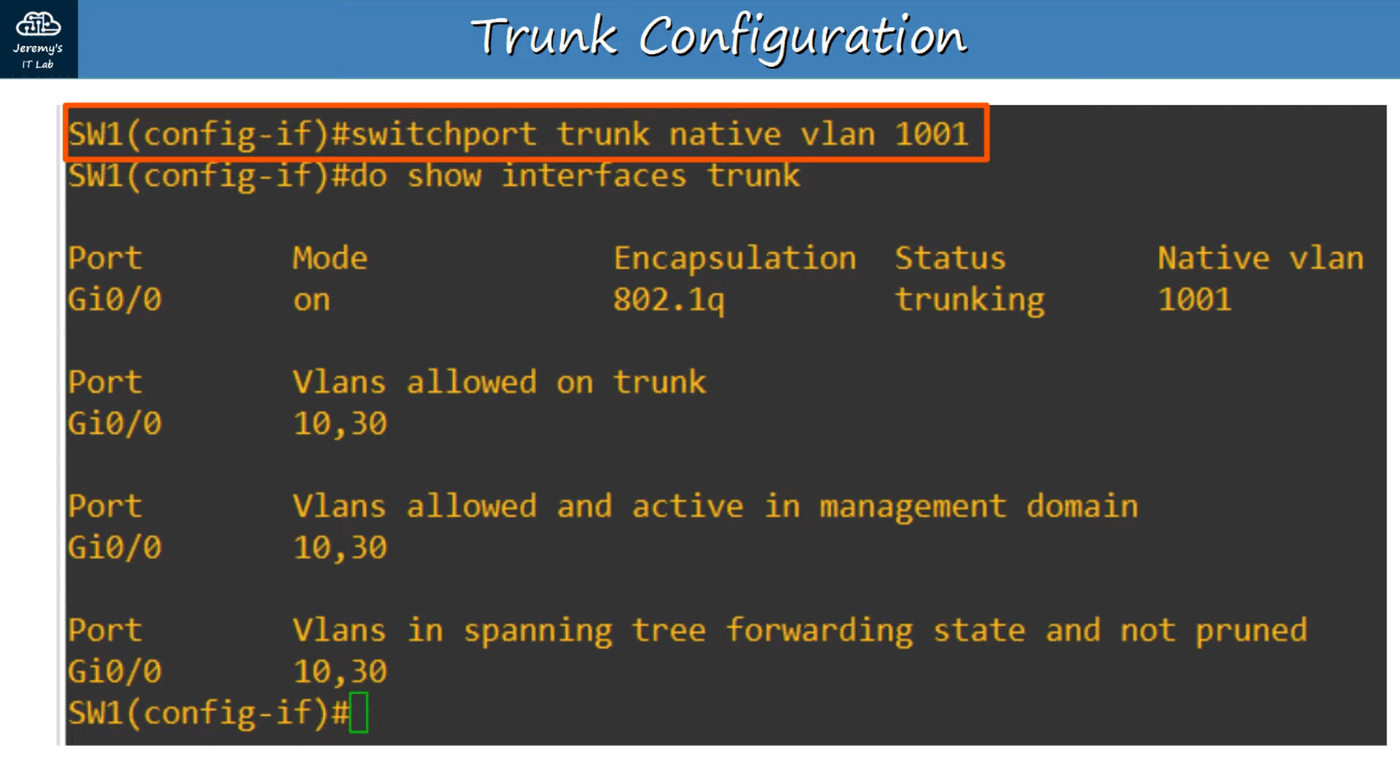
\includegraphics[keepaspectratio,alt={image}]{images/18-vlan-part2/img-017.png}}
\end{figure}

\begin{figure}
\centering
\pandocbounded{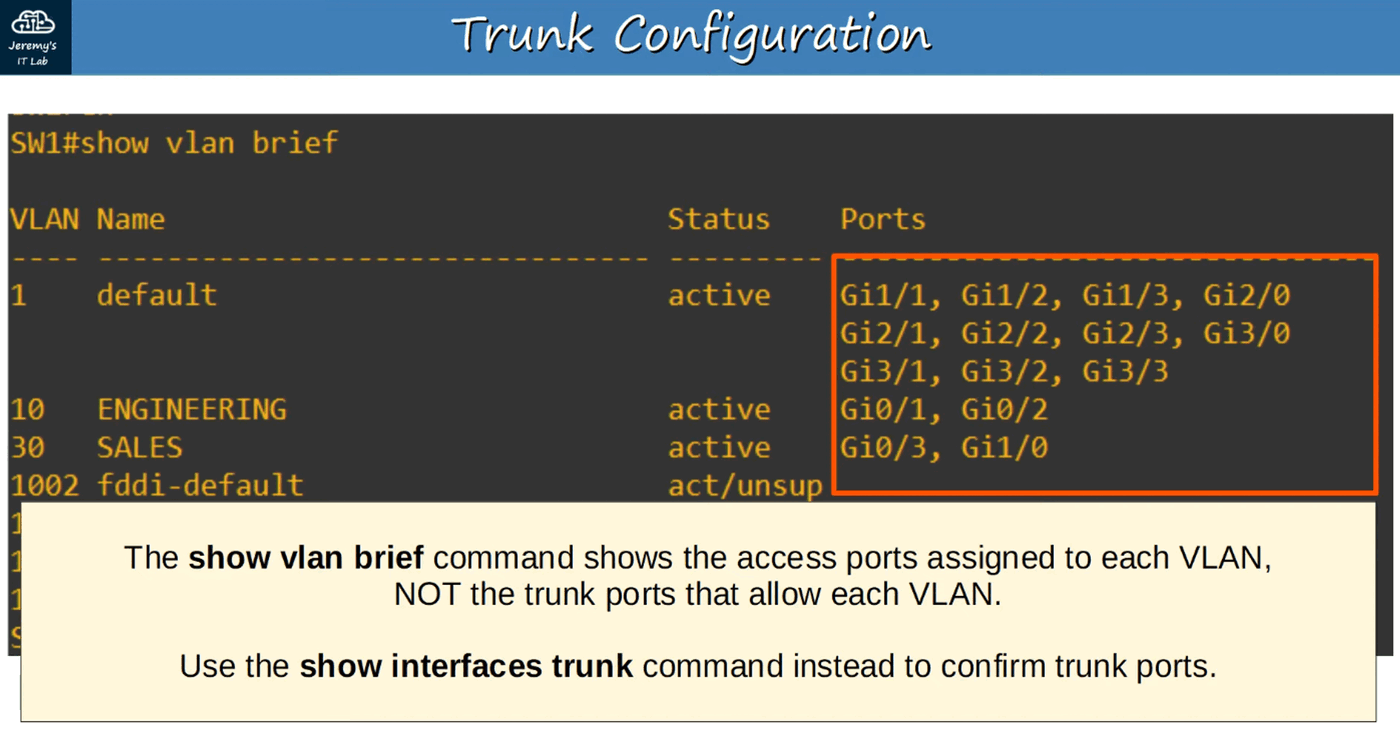
\includegraphics[keepaspectratio,alt={image}]{images/18-vlan-part2/img-018.png}}
\end{figure}

Setting up our TRUNKS for this Network

\begin{figure}
\centering
\pandocbounded{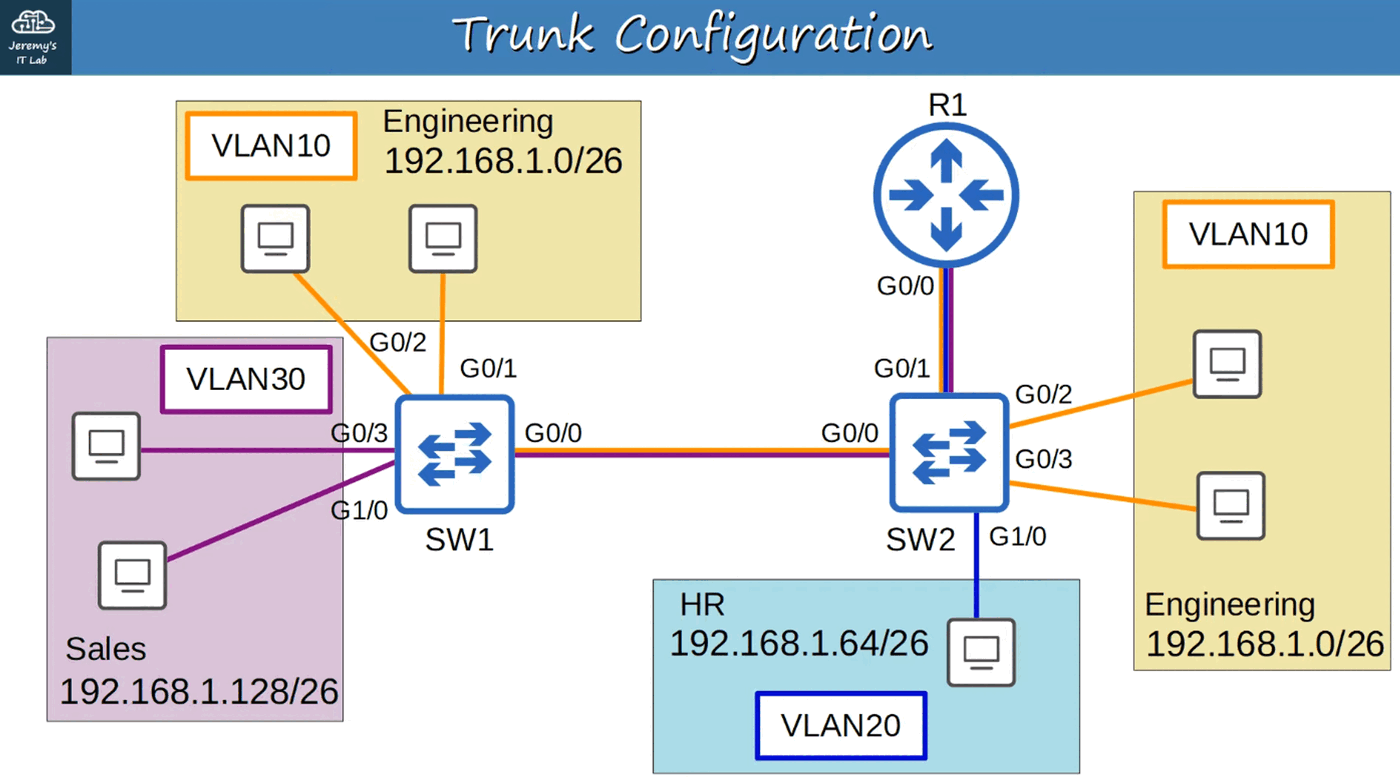
\includegraphics[keepaspectratio,alt={image}]{images/18-vlan-part2/img-019.png}}
\end{figure}

We will need to configure :

SW1 : g0/0 interface (already configure above this section)

SW2: g0/0, and g0/1 interface

SW2 g0/0

\begin{figure}
\centering
\pandocbounded{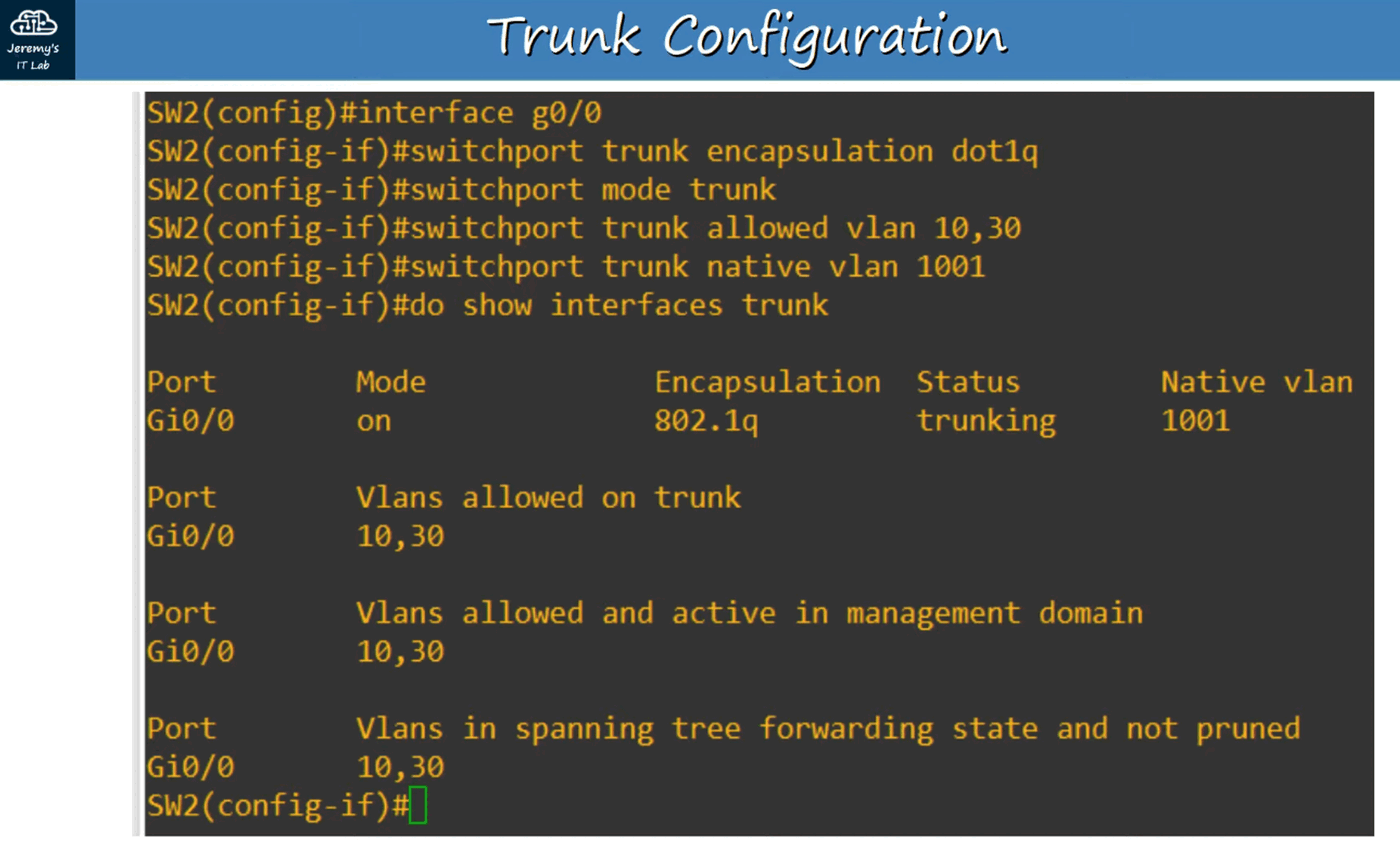
\includegraphics[keepaspectratio,alt={image}]{images/18-vlan-part2/img-020.png}}
\end{figure}

SW2 g0/1

\begin{figure}
\centering
\pandocbounded{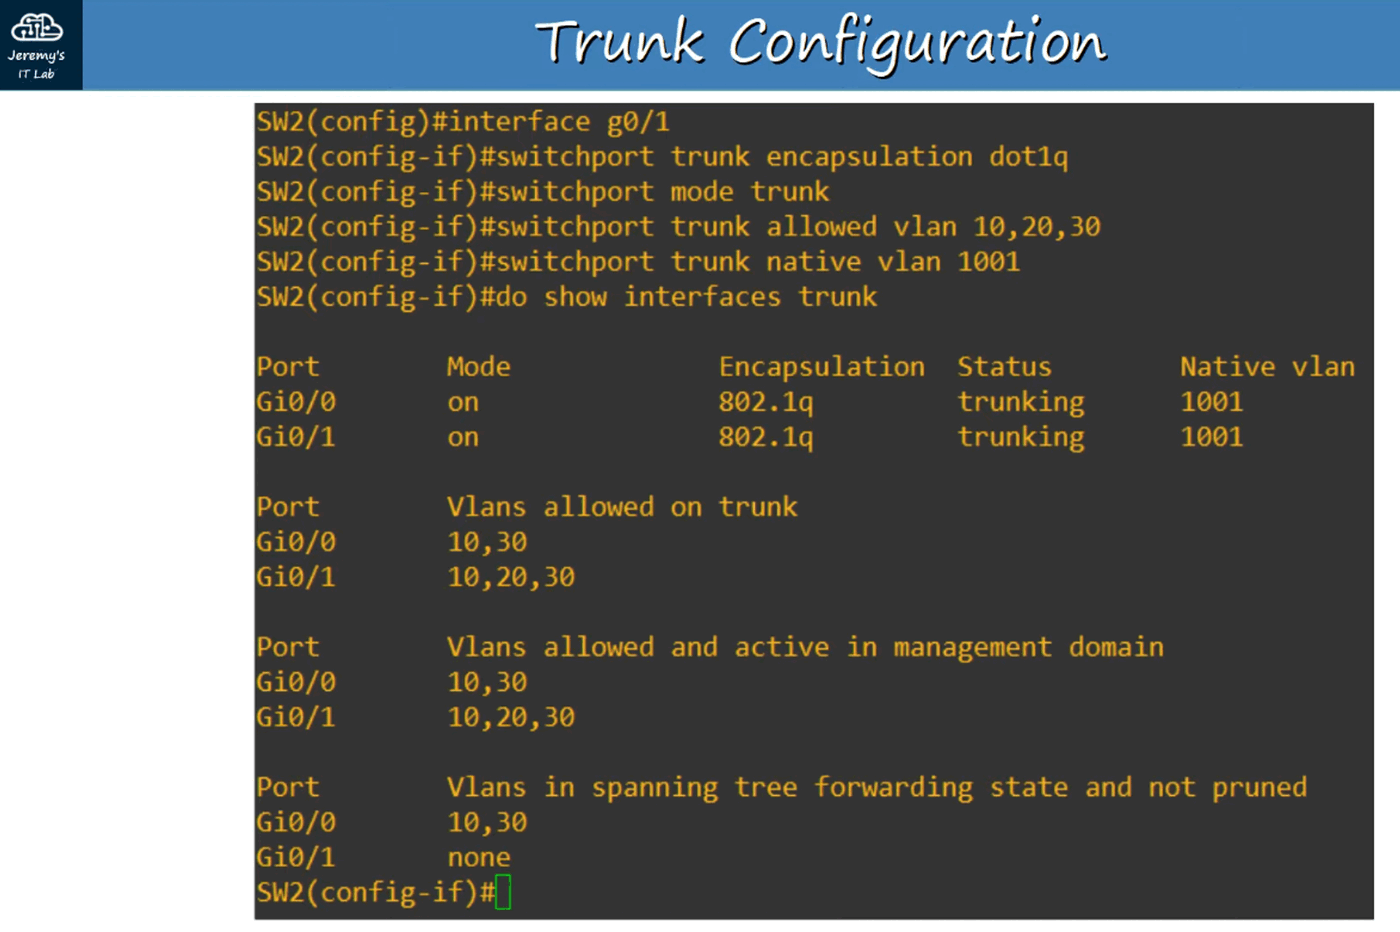
\includegraphics[keepaspectratio,alt={image}]{images/18-vlan-part2/img-021.png}}
\end{figure}

What about the ROUTER, R1 ?

\section{Router on a Stick (ROAS)}\label{router-on-a-stick-roas}

\begin{figure}
\centering
\pandocbounded{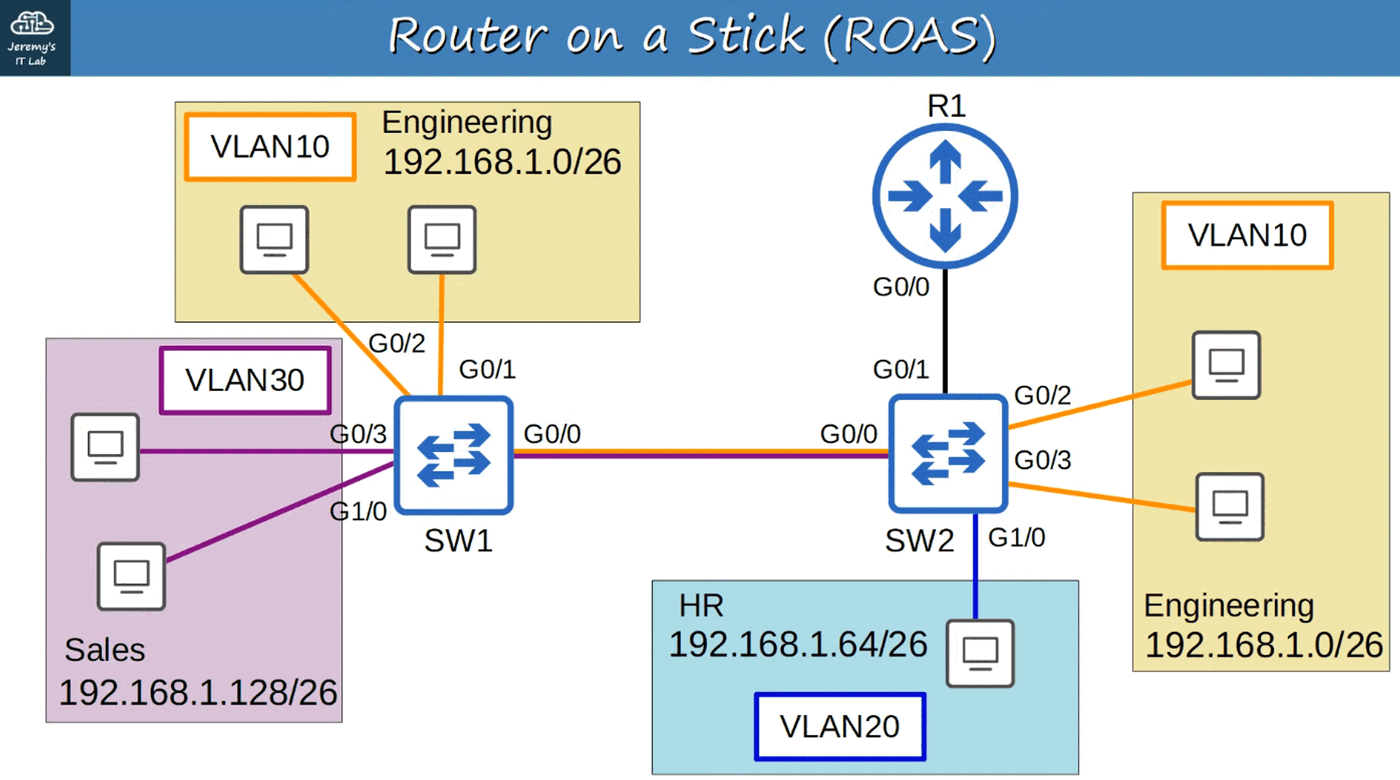
\includegraphics[keepaspectratio,alt={image}]{images/18-vlan-part2/img-022.png}}
\end{figure}

\begin{figure}
\centering
\pandocbounded{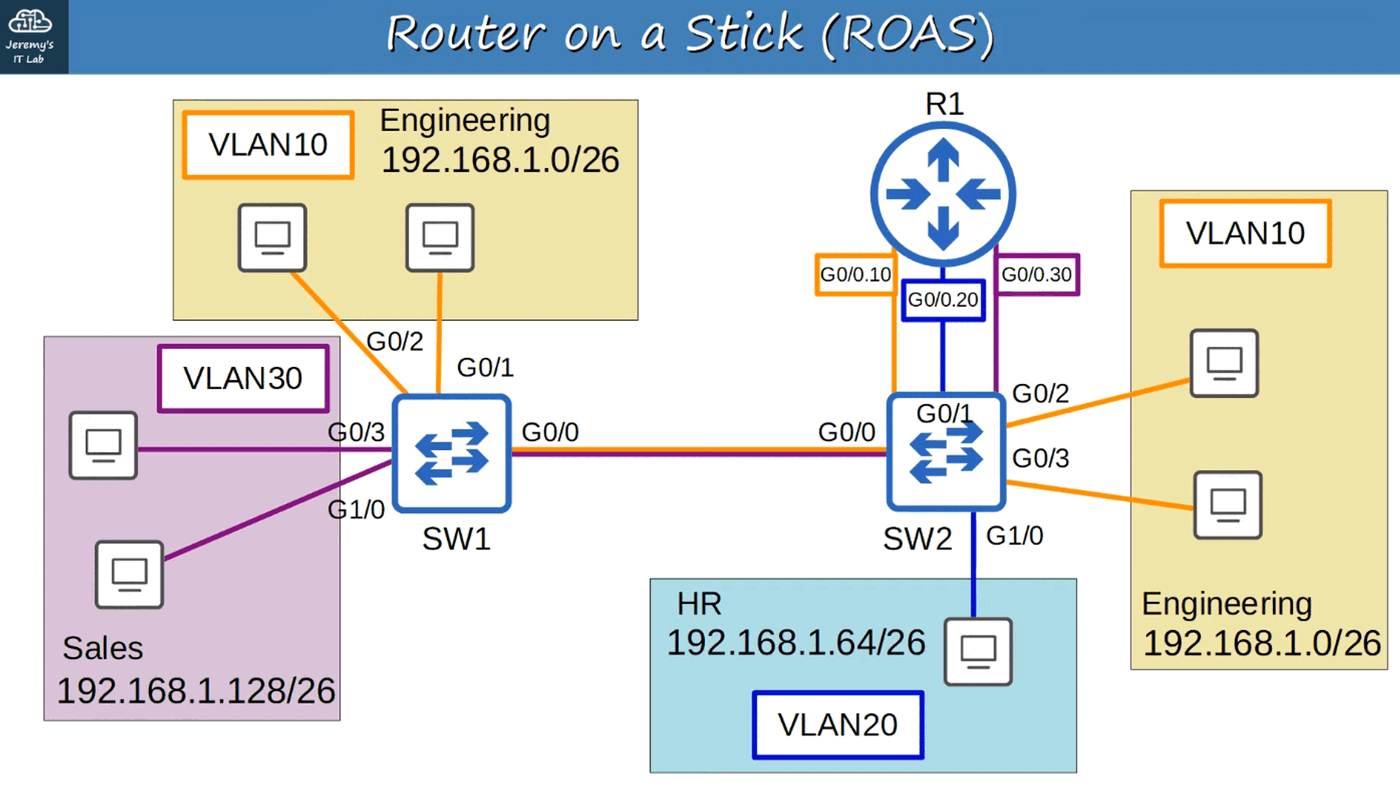
\includegraphics[keepaspectratio,alt={image}]{images/18-vlan-part2/img-023.png}}
\end{figure}

\begin{figure}
\centering
\pandocbounded{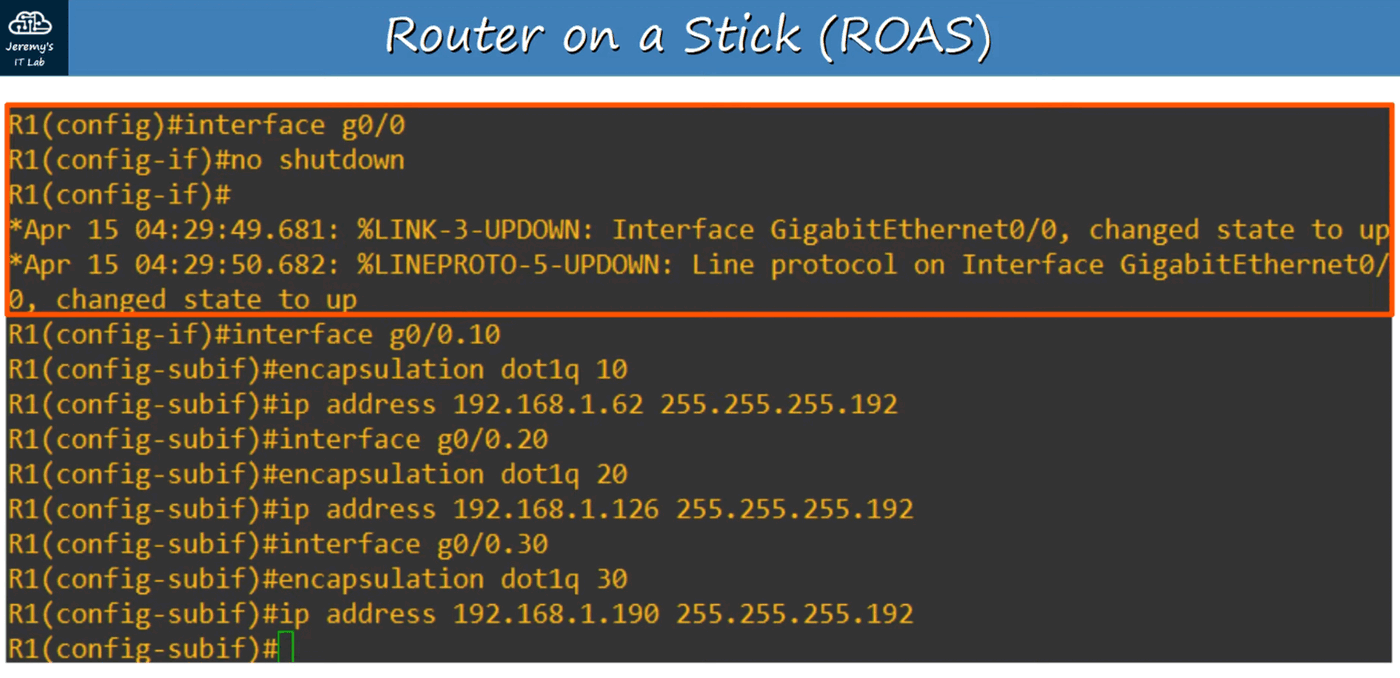
\includegraphics[keepaspectratio,alt={image}]{images/18-vlan-part2/img-024.png}}
\end{figure}

NOTE the Sub-Interface names (like the network diagram) of 0.10, 0.20
and 0.30

You assign them IP addresses identically like you would a regular
interface (using the last usable IP address of a given VLAN subnet)

Sub-interfaces will appear with the ``show ip interface brief'' command

\begin{figure}
\centering
\pandocbounded{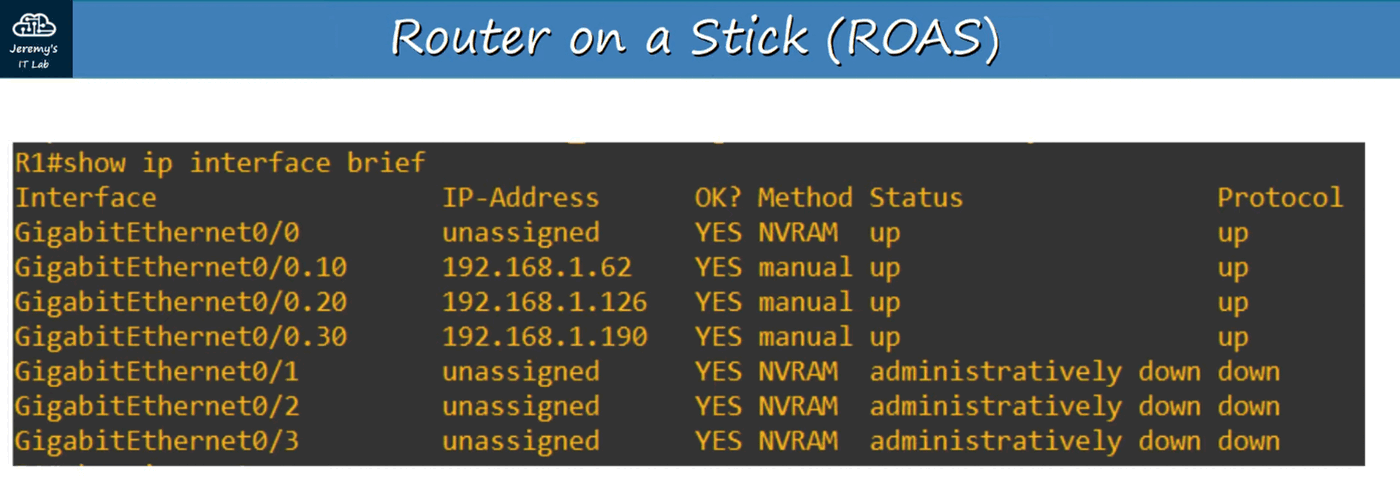
\includegraphics[keepaspectratio,alt={image}]{images/18-vlan-part2/img-025.png}}
\end{figure}

They also appear in the ``show ip route'' command (Route Table)

\begin{figure}
\centering
\pandocbounded{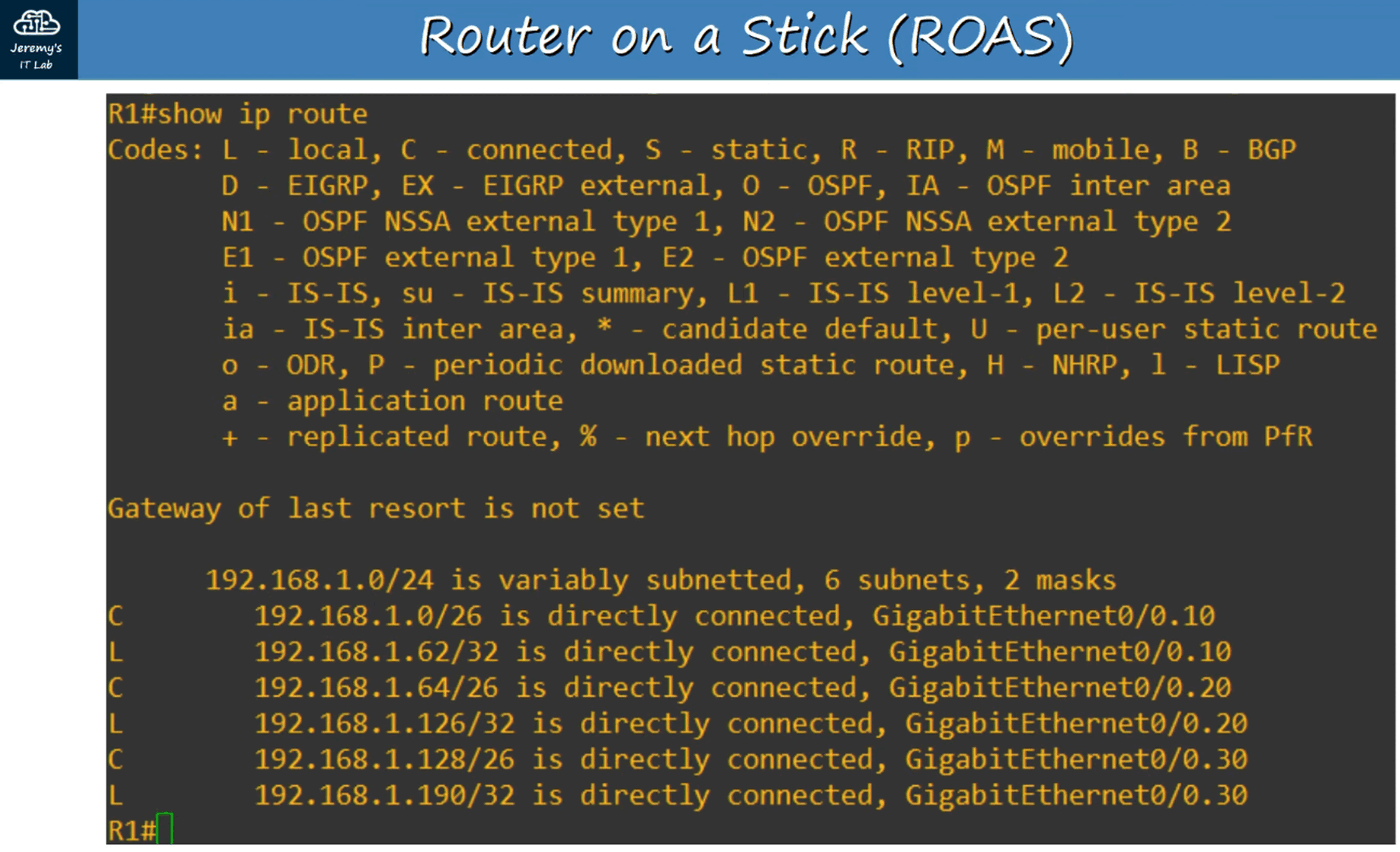
\includegraphics[keepaspectratio,alt={image}]{images/18-vlan-part2/img-026.png}}
\end{figure}

ROAS is used to route between multiple VLANs using a SINGLE interface on
a ROUTER and SWITCH

The SWITCH interface is configured as a regular TRUNK

The ROUTER interface is configured using SUB-INTERFACES. You configure
the VLAN tag and IP address on EACH SUB-INTERFACE

The ROUTER will behave as if frames arriving with a certain VLAN tag
have arrived on the SUB-INTERFACE configured with that VLAN tag

The ROUTER will TAG frames sent out of EACH SUB-INTERFACE with the VLAN
TAG configured on the SUB-INTERFACE
